% supplementary.tex -- supplementary figures.
%
% Placed AFTER the bibliography (user, 2026-10-05): these were previously inside
% Materials and Methods, ahead of the references, so the paper had no supplementary
% section at all. The figure counter is reset and prefixed with S here, so these
% render as Figure S1, S2, ... rather than continuing the main sequence at 6.
%
% ASSEMBLY RULE -- NOW SATISFIED FOR S1-S3 (2026-10-05). Each supplementary figure
% is ONE pdf assembled in Illustrator from individually exported jn-style panels,
% exactly like the main figures -- never several \includegraphics stitched with
% \hfill. S1.pdf, S2.pdf and S3.pdf are those assemblies; the panels they are built
% from live in brain_paper/paper/figures_final/panels/ and are listed in
% MANIFEST.txt. Do not re-introduce multi-\includegraphics figures here.
%
% These three assemblies replace seven earlier floats:
%   S1 <- imp_spatial_area + imp_spatial_maps + spont_variance, plus the new
%         onset-variance panel. The standalone spont_variance float is gone and
%         fig:spont_variance now resolves to S1C.
%   S2 <- grid_cost_surface_AL_0033_0305 + grid_cost_surface_AL_0034_1017
%         + autotune_convergence_both. The AL_0034 grid panel was CUT: the pair now
%         shown is one mouse (AL_0033) across two sessions, which is what makes the
%         grid/auto-tune agreement a cross-check rather than a coincidence of rigs.
%   S3 <- f4_exemplars_sessions + the three f4_decomp_unique panels.
% Panel letters moved, so every \ref to these labels now carries a letter. If a
% panel is re-lettered in Illustrator, grep the whole manuscript for the label.

\clearpage
\section*{Supplementary figures}
\setcounter{figure}{0}
\renewcommand{\thefigure}{S\arabic{figure}}

\begin{figure}[h]
    \centering
    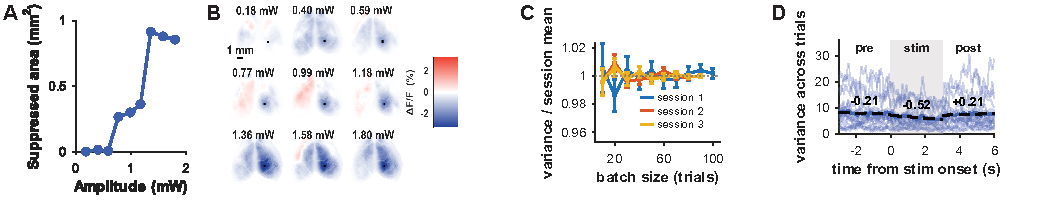
\includegraphics[width=\linewidth]{images/supplementary/S1.pdf}
    \caption{\textbf{Spatial spread of optogenetic inhibition, and the validity of
    trial averaging.}
    \textbf{A:} Suppressed area against stimulation amplitude
    (AL\_0033, 2025-01-29). A pixel counts as suppressed if its
    background-corrected response falls below half the median response within
    $0.2$\,mm of the peak at the strongest amplitude; background is the mean over
    an annulus $0.6$--$0.9$\,mm from that peak. Areas are therefore relative to
    the response at the strongest amplitude.
    \textbf{B:} Trial-averaged $\Delta F/F$ (\%) over 0--200\,ms post-onset at each
    of the nine delivered amplitudes, masked to the brain, on a symmetric
    blue--white--red scale (zero white, suppression blue). Black
    square, a $10\times10$\,pixel box, the size of the readout kernel, centered on
    the suppression peak. Scale
    bar, $1$\,mm (pixel scale $0.0173$\,mm).
    \textbf{C:} Total cross-trial variance of spontaneous $\Delta F/F$ against the
    number of trials $N$ entering the average, for three of the closed-loop
    sessions, each divided by its own mean over $N$. Points, means over 500 random
    subsamples per batch size; error bars, SEM; dotted line, 1. Batch sizes at or above
    the full trial count of a session are omitted.
    \textbf{D:} Across-trial variance of $\Delta F/F$ against time from stimulation
    onset for open-loop trials. Thin lines, individual sessions; bold line and
    shading, mean $\pm$ SEM across sessions; gray band, the 3\,s stimulation
    window. Dashed lines, least-squares fits within the pre-stimulus,
    stimulation and post-stimulus epochs, labeled with their slopes (variance per
    second).}
    \label{fig:spatial_spread}
\end{figure}

\begin{figure}[!ht]
    \centering
    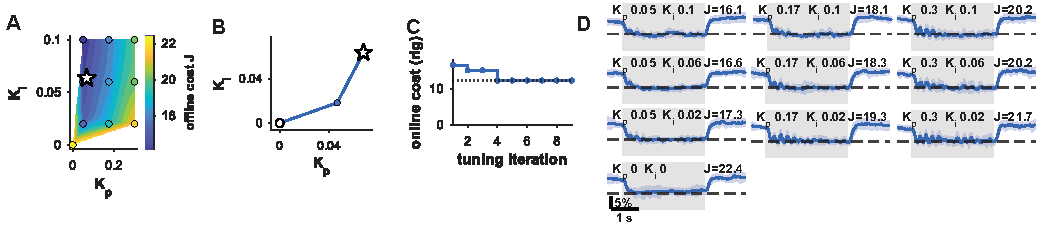
\includegraphics[width=\linewidth]{images/supplementary/S2.pdf}
    \caption{\textbf{Controller gain tuning.} All panels are from one mouse
    (AL\_0033): the grid sweep on 2025-03-05 and the auto-tuning session on
    2025-03-17.
    \textbf{A:} Empirical cost surface $\hat{J}(K)$ over the grid of fixed PI
    gains, interpolated between the occupied nodes (circles); star, the final
    gains accepted in the auto-tuning session (as in \textbf{B}).
    \textbf{B:} The gain pairs accepted by the online zeroth-order search in the
    separate auto-tuning session, from the open-loop start at $K_p = K_i = 0$
    (open circle) to the final accepted gains (star).
    \textbf{C:} Running cost over tuning iterations in that session; dotted line,
    the final accepted cost.
    \textbf{D:} Trial-averaged closed-loop response at each grid node, labeled with
    its gains and its cost $\hat{J}$, including the $K_p = K_i = 0$
    feedforward-only node. Mean (bold) $\pm$ 1 SD across trials; dashed line,
    reference ($-5\%\,\Delta F/F$); shading, stimulation window; scale bars 1\,s
    and 5\%.
    $\hat{J}$ in \textbf{A} and \textbf{D} is scored offline over
    $t = 0$ to $+3$\,s. The cost in \textbf{C} is the cost the rig computed online
    over the stimulation window less two samples, so its absolute values are not
    comparable with \textbf{A} and \textbf{D}.}
    \label{fig:cost_landscape}
\end{figure}

\begin{figure}
    \centering
    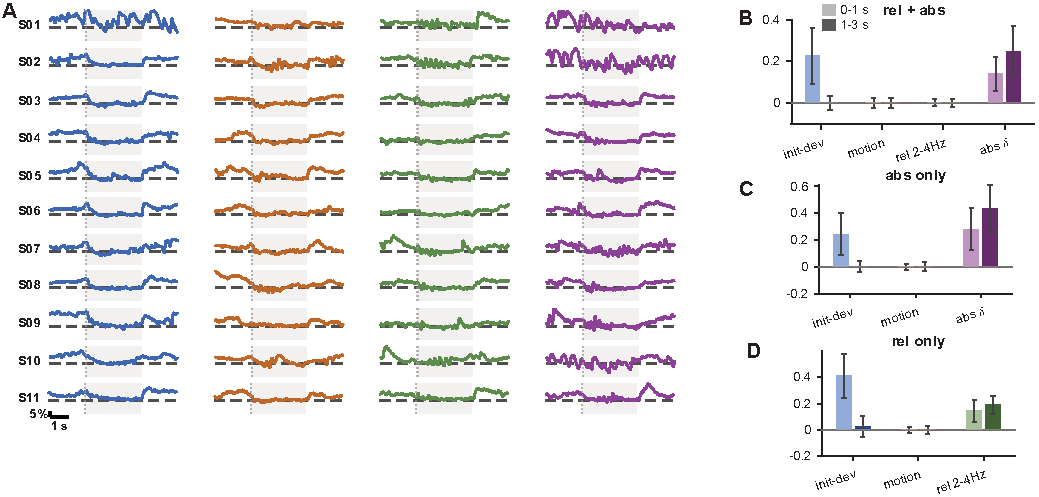
\includegraphics[width=\linewidth]{images/supplementary/S3.pdf}
    \caption{\textbf{State exemplars for every session, and the error decomposition under
    three definitions of the low-frequency factor.}
    \textbf{A:} For every session with motion capture (rows), a representative
    closed-loop trial for each of four state measures (columns: high initial
    deviation, high motion, high relative 2--4\,Hz power, high absolute 1--4\,Hz
    power), chosen as the trial highest in that state and low in the others within
    that session (Materials and Methods, \emph{State exemplars and error
    decomposition}). Colors match
    Fig.~\ref{fig:figure4}A. Dashed line, reference ($-5\%\,\Delta F/F$); shading,
    stimulation window; scale bars 1\,s and 5\%.
    \textbf{B--D:} Unique $R^2$ of each state factor for closed-loop tracking
    error, in the transient (0--1\,s, light) and steady-state (1--3\,s, dark)
    windows, under three specifications of the low-frequency term: relative
    2--4\,Hz and absolute 1--4\,Hz power entered together in one model
    (\textbf{B}), absolute only (\textbf{C}), and relative only (\textbf{D}).
    Bars, unique $R^2$ on trials pooled across sessions; error bars, 1 SD across
    sessions. Fig.~\ref{fig:figure4}C takes initial deviation, motion and the
    relative term from \textbf{D} and the absolute term from \textbf{C}.}
    \label{fig:f4_exemplars}
\end{figure}

%% TABLED (user 2026-10-10: not in the paper for now). Single-trial A-r vs D figure;
%% producer controller-analysis/f4_supp_reject_trials.m. Uncomment to restore, and
%% restore the two Discussion cross-references (see brain_paper RESEARCH 2026-10-10).
% \begin{figure}
%     \centering
%     %% ASSEMBLY PENDING. Place the four panels from
%     %% paper/figures_final/panels/supp_reject/ (each 11.15 x 5.33 cm, stack as four
%     %% rows A-D) and export as images/supplementary/S4.pdf, then uncomment the line
%     %% below. Caption, label and the Discussion cross-reference are already live, so
%     %% the draft builds with a caption-only float until the artwork lands.
%     % \includegraphics[width=\linewidth]{images/supplementary/S4.pdf}
%     \caption{\textbf{Single trials behind the rejection ratio.} Each tile is one
%     trial and draws the two traces whose energies form the rejection ratio of
%     Fig.~\ref{fig:figure4}G, on a common zero baseline. Color, the tracking error
%     $A - r$ (red, open loop; blue, closed loop); dashed line, zero error, i.e.\ the
%     response on the reference $r = -5\%\,\Delta F/F$. Grey, the disturbance $D$:
%     the stimulation-blind contralateral prediction referenced to its own 1\,s
%     pre-stimulus baseline, minus the session-mean open-loop laser leak while the
%     laser is on (blue bar, 0--3\,s). Grey band, the settled window 1--3\,s; traces are
%     drawn at full strength only there, because these are the only samples
%     $\mathrm{RR} = \lVert A - r\rVert^2 / \lVert D\rVert^2$ uses. Lighter traces, from
%     3\,s before onset to 2\,s after the laser turns off, are context only. Each
%     panel shows one session as two rows, open loop above and closed loop below,
%     with three trials drawn at the 10th, 50th and 90th percentiles of that
%     session's ratio, so each row spans the session's range rather than its best
%     trials; all six tiles in a panel share one $y$-range. Each printed
%     $\mathrm{RR}$ is one of the trials inside the Fig.~\ref{fig:figure4}G
%     statistic. \textbf{A--C:} Three sessions from the analysed pool, one per mouse
%     (AL\_0033 2025-02-26, AL\_0039 2025-04-20, AL\_0048 2026-07-29; session-median
%     $\mathrm{RR} = 0.72$, $0.74$ and $0.75$ closed loop against $1.26$, $1.25$ and
%     $0.84$ open loop). Within the window the closed-loop error stays smaller than
%     the disturbance it faces, whereas the open-loop error carries the disturbance
%     plus a standing displacement from the reference. \textbf{D:} AL\_0051
%     2026-07-29, the session excluded because its standing setpoint offset supplies
%     $59\%$ of its settled residual (Materials and Methods). Its closed-loop error
%     sits persistently above zero even where the disturbance is near zero, which is
%     the failure the exclusion criterion is meant to identify.}
%     \label{fig:reject_trials}
% \end{figure}

\begin{figure}
    \centering
    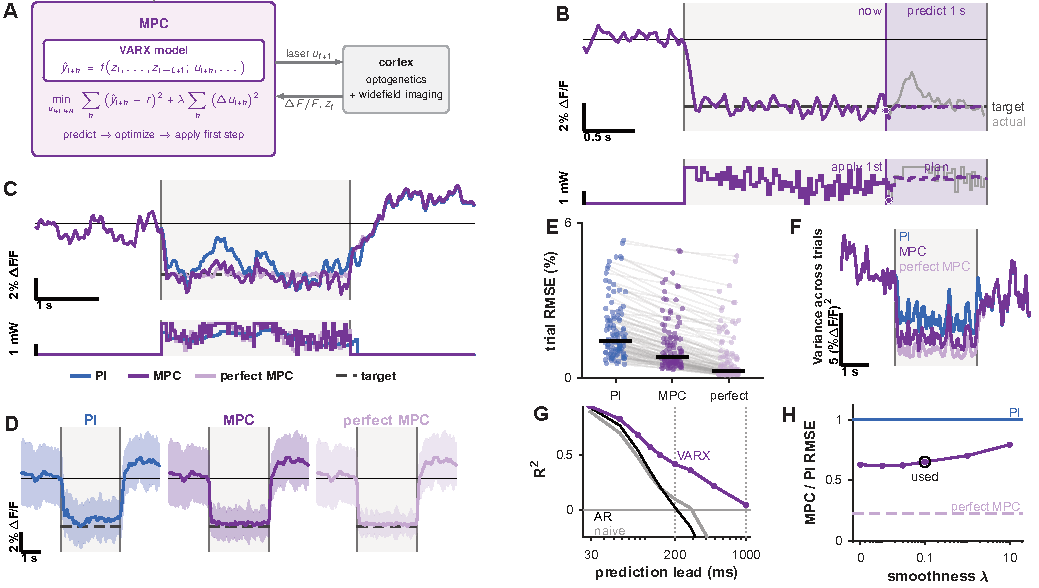
\includegraphics[width=\linewidth]{images/supplementary/S_mpc.pdf}
    \caption{\textbf{A model-predictive controller outperforms the recorded PI controller
    in simulation.} One session
    (AL\_0033 2025-02-26, 108 closed-loop trials). All values come from simulation
    and are descriptive; no statistical tests were applied.
    \textbf{A:} The controller. At every frame (35\,Hz) the MPC reads $\Delta F/F$
    at the controlled site and at 100 sites spread over dorsal cortex ($z_t$),
    predicts the controlled signal $\hat y$ over a horizon $H = 1$\,s for a
    candidate plan of laser commands, and chooses the plan that minimizes the
    squared deviation from the target $r$ plus a penalty $\lambda$ on command
    changes $\Delta u$ (with a small penalty on departures from the steady-state
    command and within the rig's command limits; $\lambda = 0.1$). It applies the
    first command and solves again at the next frame. The predictor is a vector
    autoregressive model with exogenous laser input (VARX; ten lags, 286\,ms),
    fitted by ridge regression.
    \textbf{B:} One MPC step on a closed-loop trial, 2.0\,s after stimulus onset.
    Purple, the controlled signal and laser command up to that moment; dashed,
    the predicted signal and the planned command over the next 1\,s (shaded);
    grey, what happened next.
    \textbf{C:} The trial at the median of the per-trial MPC improvement. Blue, the
    recorded PI trial; purple, MPC; light purple, the same MPC given the future
    residuals of the simulated cortex (perfect prediction). Lower traces, laser
    command. Grey band, stimulation; dashed line, reference ($-5\%\,\Delta F/F$).
    \textbf{D:} Trial average $\pm$ SD over the 108 trials.
    \textbf{E:} Per-trial RMSE over the settled window (1--3\,s). Lines join the
    same trial; black bars, medians.
    \textbf{F:} Variance across trials over time. The three traces share the
    recorded trials before onset, and the simulated laser is off after the
    stimulation ends.
    \textbf{G:} Prediction $R^2$ of the controlled signal against lead time on 92
    held-out open-loop trials (five folds), for the VARX, a univariate
    autoregressive model (AR; order 35, chosen on validation data) of the kind
    benchmarked on spontaneous widefield activity by \citet{lu2025benchmarking},
    and the last observed value (naive). Dotted lines, 200\,ms and 1\,s.
    \textbf{H:} Median ratio of MPC to PI RMSE against the command-smoothness
    penalty $\lambda$; circle, the value used ($\lambda = 0.1$); solid line, PI;
    dashed line, MPC with perfect prediction.
    The simulated cortex is the VARX fitted to all data and driven by each trial's
    recorded one-step residuals. Under the recorded laser it reproduces the recorded
    trial exactly, so the PI baseline is the recorded trial itself and needs no
    model of the PI loop. The MPC's own VARX was fitted with that trial's fold held
    out (five folds).}
    \label{fig:mpc_direct}
\end{figure}
